\chapter{\gls{fdtd} Simulation}\label{ap:fdtd_in_between}

\section{Simulation}
This appendix shows \gls{fdtd} simulation results that are out of the frequency interval used in the main part of the report. This includes the simulation plots in \autoref{sec:fdtd_simulation} illustrate strong that the cost and the beamforming filter do the array cardioid with continuous pressure in the front of the array in the hole frequency span from \SI{60}{\hertz} to \SI{300}{\hertz}



\begin{figure}[H]
\begin{subfigure}[c]{0.5\textwidth}
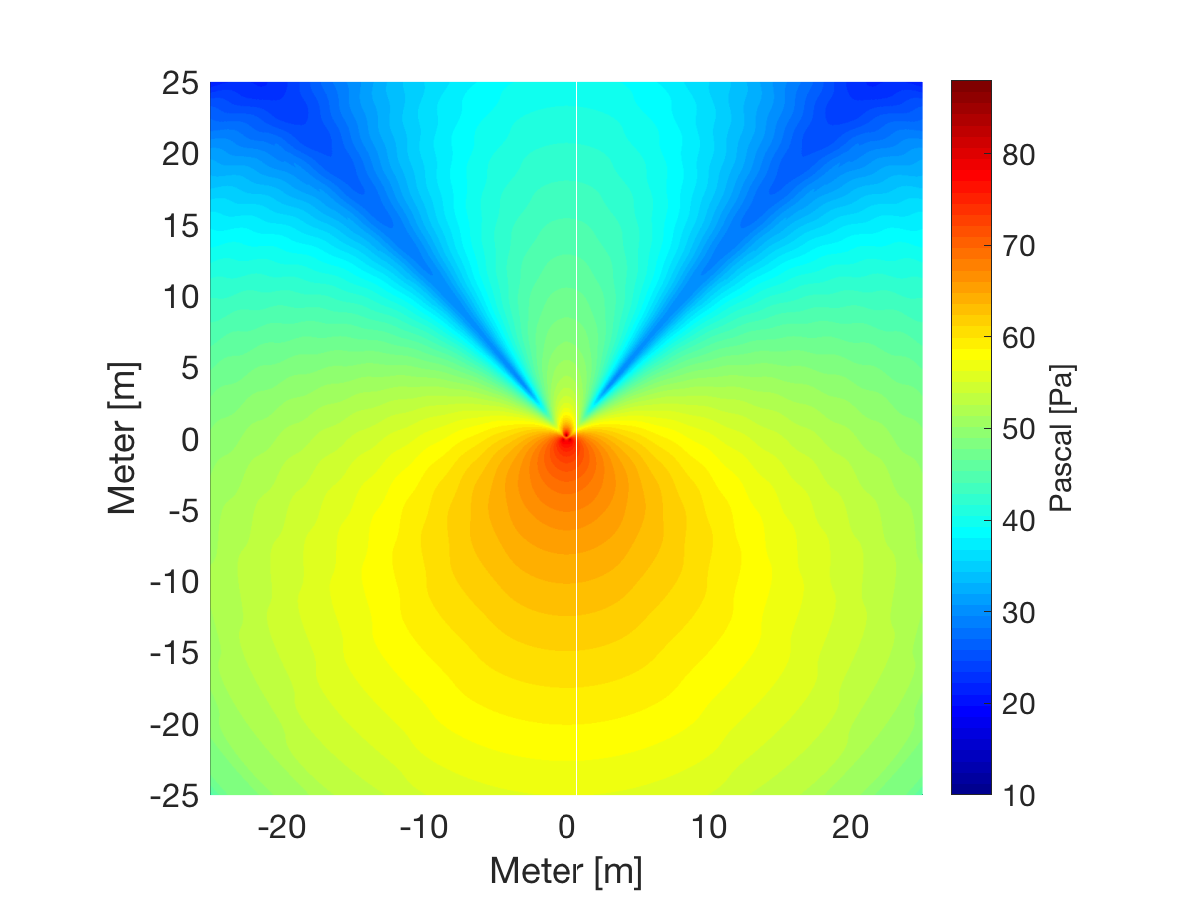
\includegraphics[width=0.95\textwidth]{70_hz_fdtd_plot.eps}
\subcaption{Simulation of  \SI{70}{\hertz}}
\label{fig:ap:fdtd_70_hz}
\end{subfigure}
\begin{subfigure}[c]{0.5\textwidth}
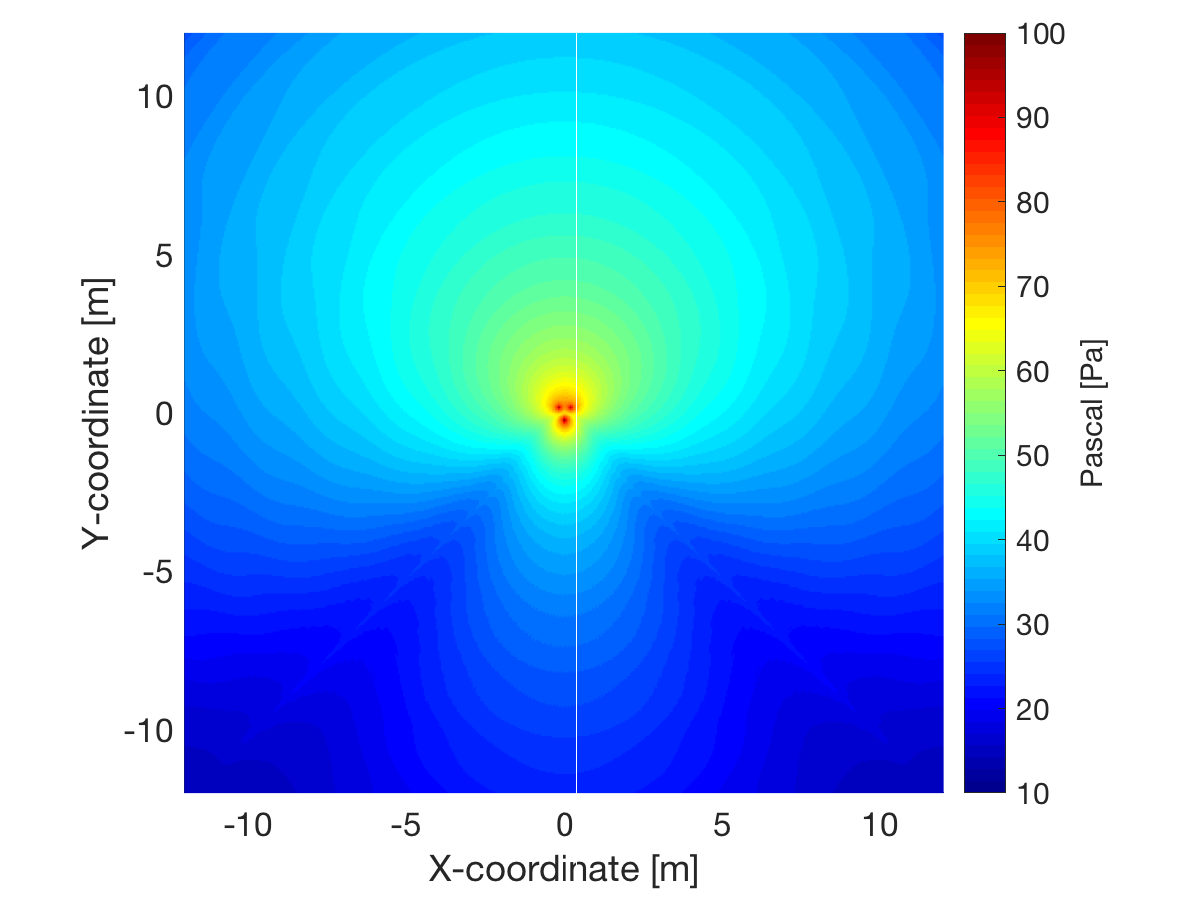
\includegraphics[width=0.95\textwidth]{80_hz_fdtd_plot.eps}
\subcaption{Simulation of  \SI{80}{\hertz}}
\label{fig:ap:fdtd_80_hz}
\end{subfigure}\\
\hspace{0.1\textheight}
\begin{subfigure}[c]{0.5\textwidth}
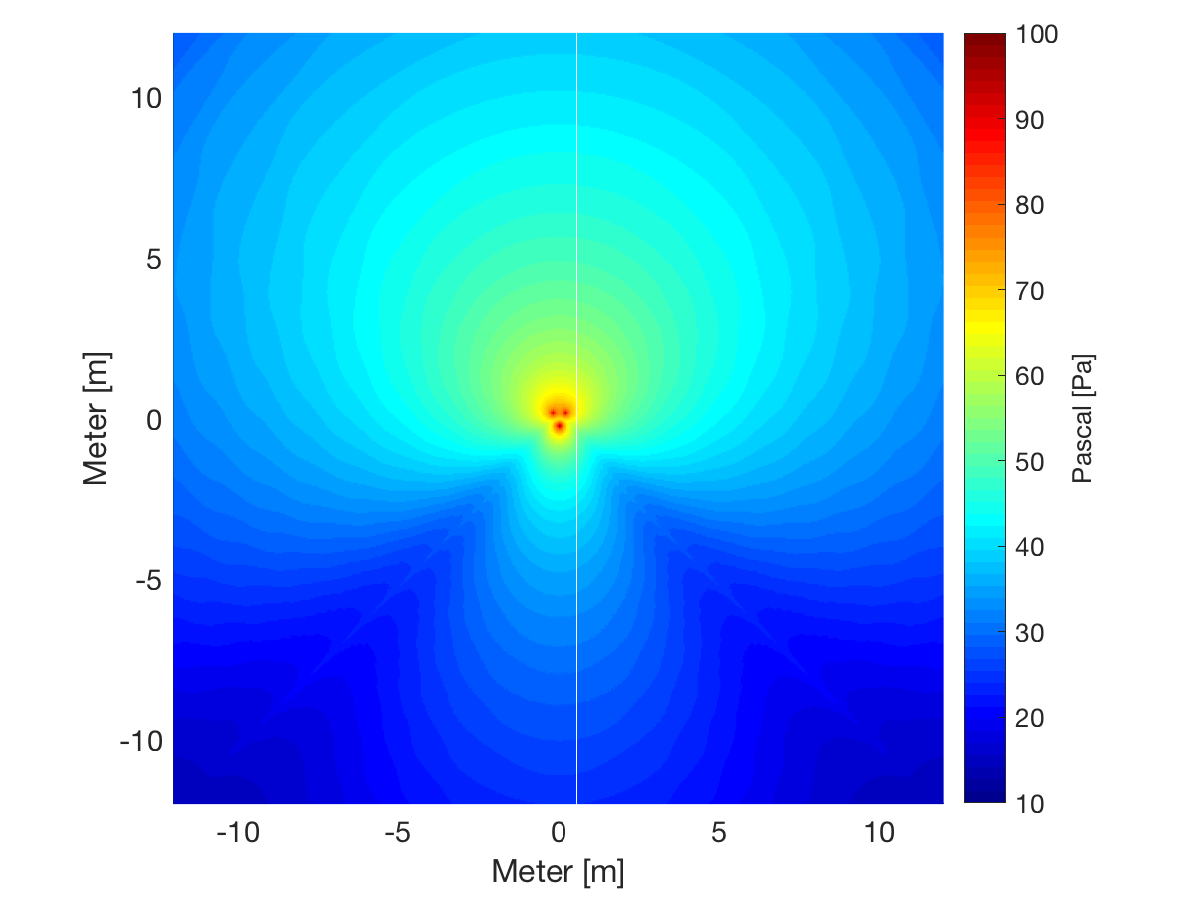
\includegraphics[width=0.95\textwidth]{120_hz_fdtd_plot.eps}
\subcaption{Simulation of  \SI{120}{\hertz}}
\label{fig:ap:fdtd_120_hz}
\end{subfigure}
\begin{subfigure}[c]{0.5\textwidth}
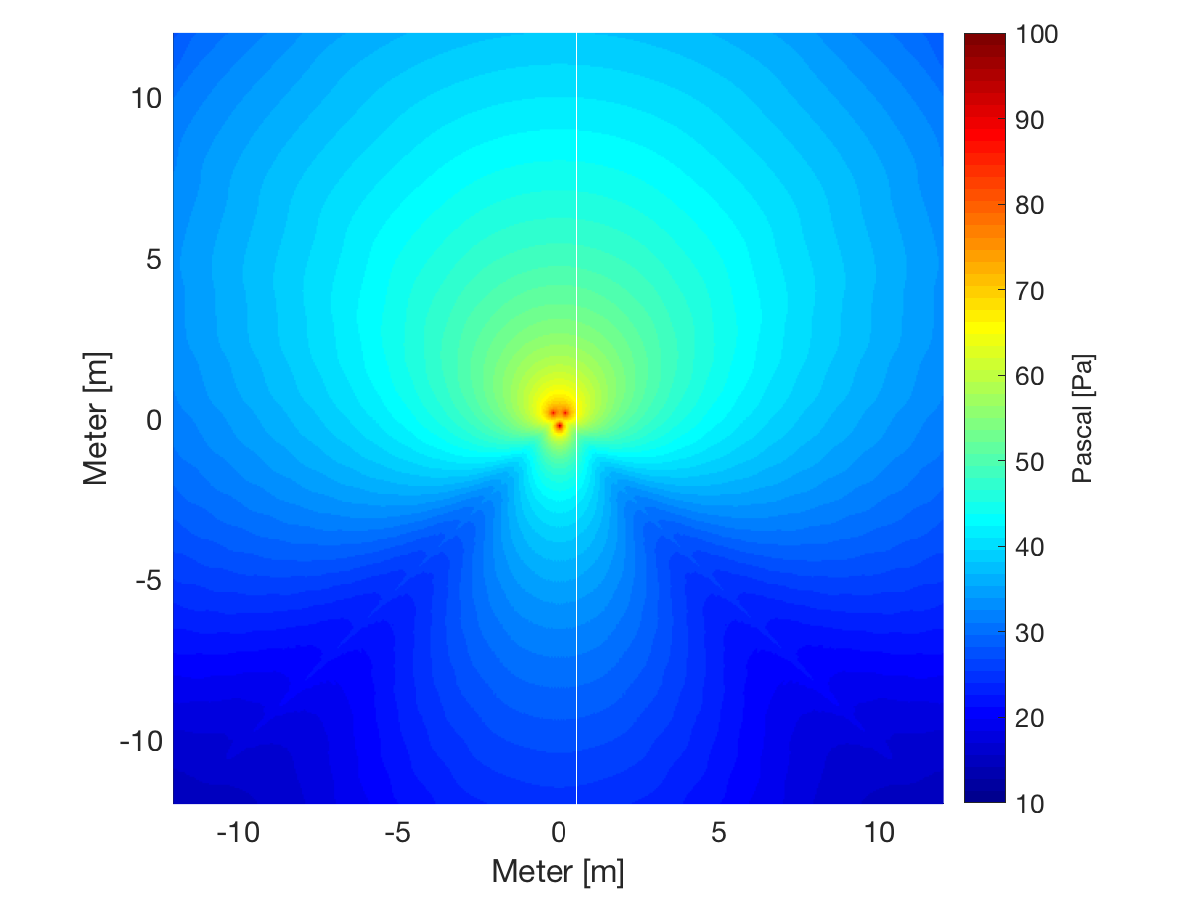
\includegraphics[width=0.95\textwidth]{180_hz_fdtd_plot.eps}
\subcaption{Simulation of  \SI{180}{\hertz}}
\label{fig:ap:fdtd_180_hz}
\end{subfigure}
\begin{subfigure}[c]{0.5\textwidth}
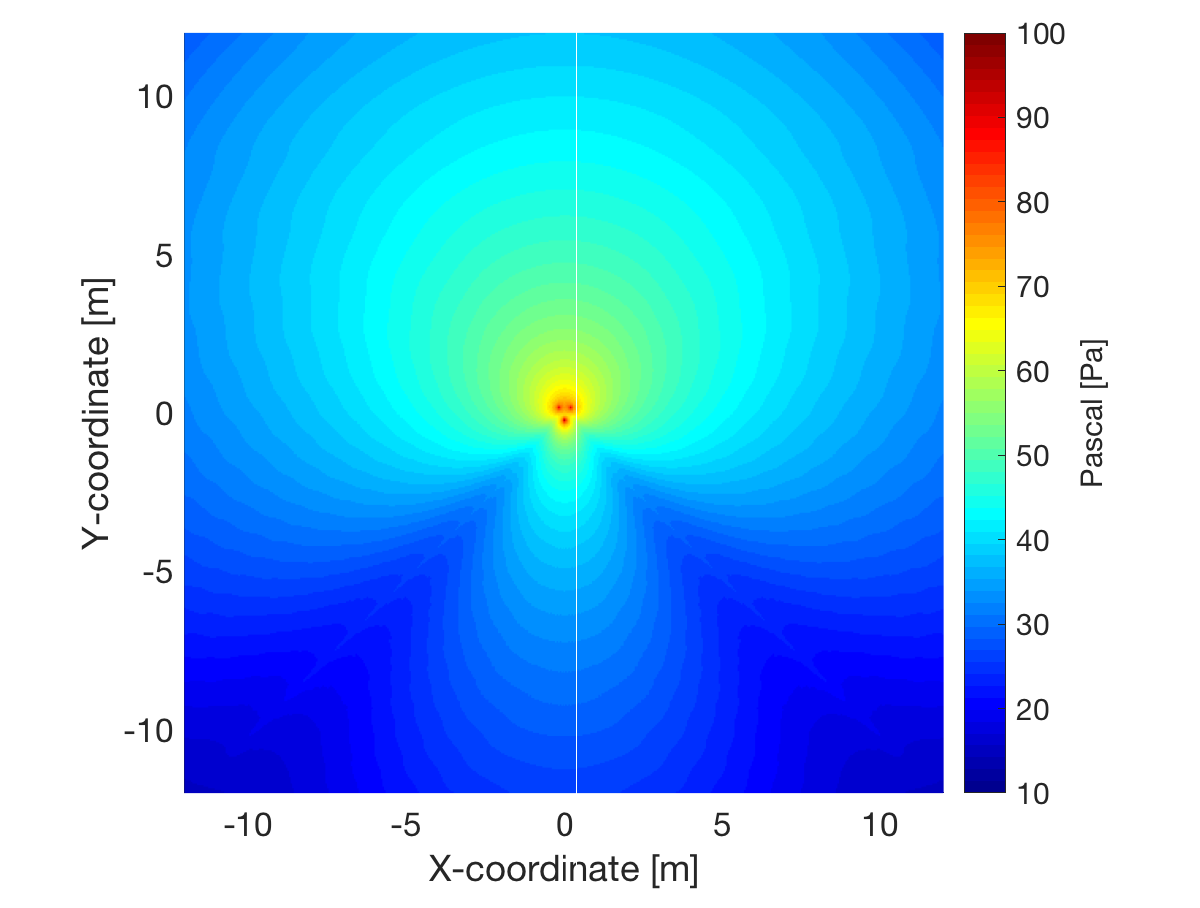
\includegraphics[width=0.95\textwidth]{220_hz_fdtd_plot.eps}
\subcaption{Simulation of  \SI{220}{\hertz}}
\label{fig:ap:fdtd_220_hz}
\end{subfigure}
\begin{subfigure}[c]{0.5\textwidth}
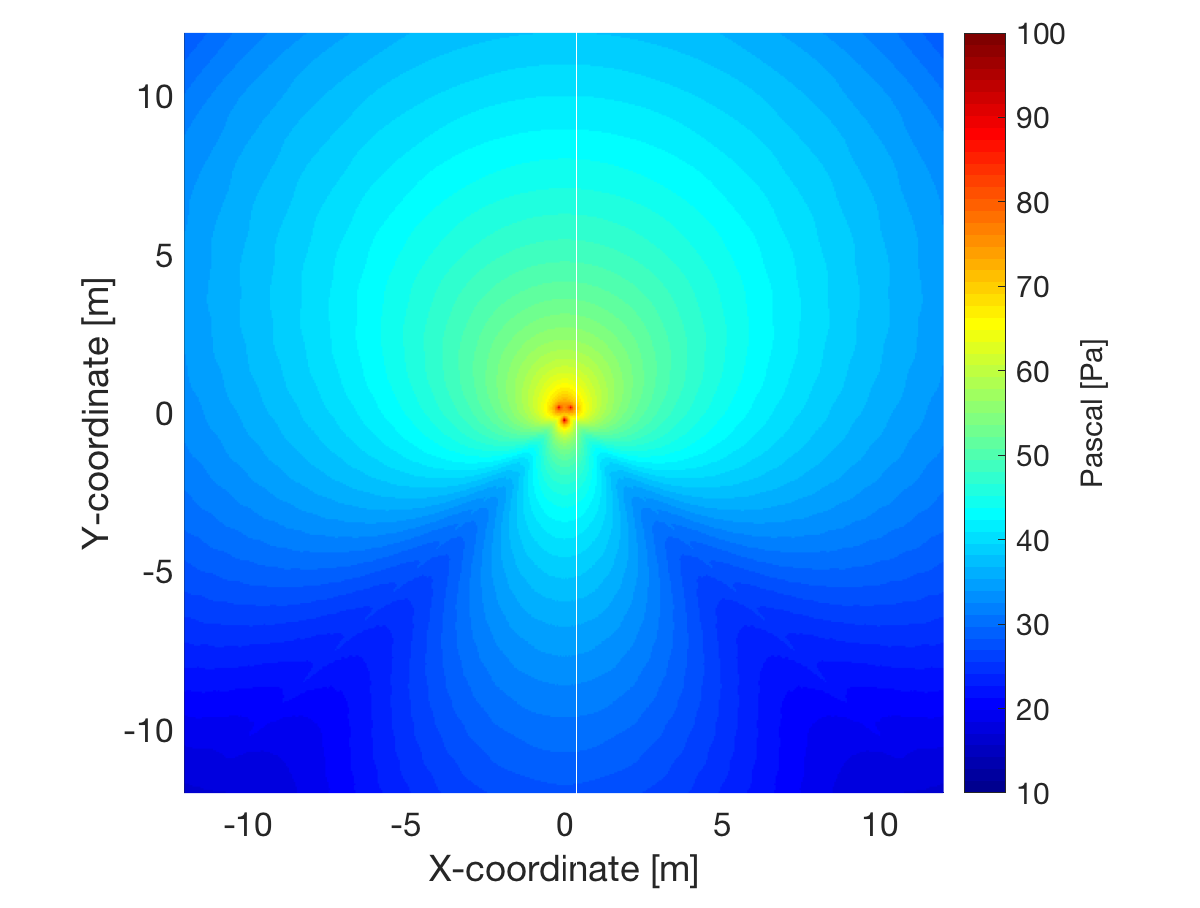
\includegraphics[width=0.95\textwidth]{280_hz_fdtd_plot.eps}
\subcaption{Simulation of  \SI{280}{\hertz}}
\label{fig:ap:fdtd_280_hz}
\end{subfigure}
\caption{The figure shows \gls{fdtd} simulation in between the used frequency range for polar plot in this project.}
		\label{fig:ap:fdtd_between}
\end{figure}

